% !TEX root = ../main.tex

\section{Online Contextualized Few-Shot Learning}
\vspace{-0.1in}
\label{sec:benchmark}
In this section, we introduce our new online contextualized few-shot learning (OC-FSL) setup in the
form of a sequential decision problem, and then introduce our new benchmark datasets.

\vspace{-0.1in}
\paragraph{Continual few-shot classification as a sequential decision problem:}
In traditional few-shot learning, an episode is constructed by a support set $S$ and a query set
$Q$. A few-shot learner $f$ is expected to predict the class of each example in the query set
$\bx^Q$ based on the support set information: $\hat{y}^Q = f(\bx^Q; (\bx^S_1, y^S_1), \dots,
(\bx^S_N, y^S_N))$, where $\bx \in \mathbb{R}^D$, and $y \in [1 \dots K]$. This setup is not a natural fit for continual learning, since it is unclear when
to insert a query set into the sequence.

Inspired by the online learning literature, we can convert continual few-shot learning into a
sequential decision problem, where every input example is also part of the evaluation: $\hat{y}_t =
f(\bx_t; (\bx_1, \tilde{y}_1), \dots, (\bx_{t-1}, \tilde{y}_{t-1}))$, for $t = 1 \dots T$, where
$\tilde{y}$ here further allows that the sequence of inputs to be semi-supervised: $\tilde{y}$
equals $y_t$ if labeled, or otherwise $-1$. The setup in \citet{mann} and \citet{rareevent} is
similar; they train RNNs using such a temporal sequence as input. However, their evaluation relies
on a ``query set'' at the end. We instead evaluate online while learning.

Figure~\ref{fig:setup}-A illustrates these features, using an example of an input sequence where an
agent is learning about new objects in a kitchen. The model is rewarded when it correctly predicts a
known class or when it indicates that the item has yet to be assigned a label.

\vspace{-0.1in}
\paragraph{Contextualized environments:}
Typical continual learning consists of a sequence of tasks, and models are trained sequentially for
each task. This feature is also preserved in many incremental learning settings~\citep{icarl}. For
instance, the split-CIFAR task divides CIFAR-100 into 10 learning environments, each with 10
classes, presented sequentially. In our formulation, the sequence returns to earlier environments
(see Figure~\ref{fig:setup}-B), which enables assessment of long-term durability of knowledge.
Although the ground-truth environment identity is not provided, we structure the task such that the
environment itself provides contextual cues which can constrain the correct class label.
\emph{Spatial} cues in the input help distinguish one environment from another. \emph{Temporal} cues
are implicit because the sequence tends to switch environments infrequently, allowing recent inputs
to be beneficial in guiding the interpretation of the current input.

\begin{figure}[t]
\centering
\vspace{-0.5in}
\iflatexml
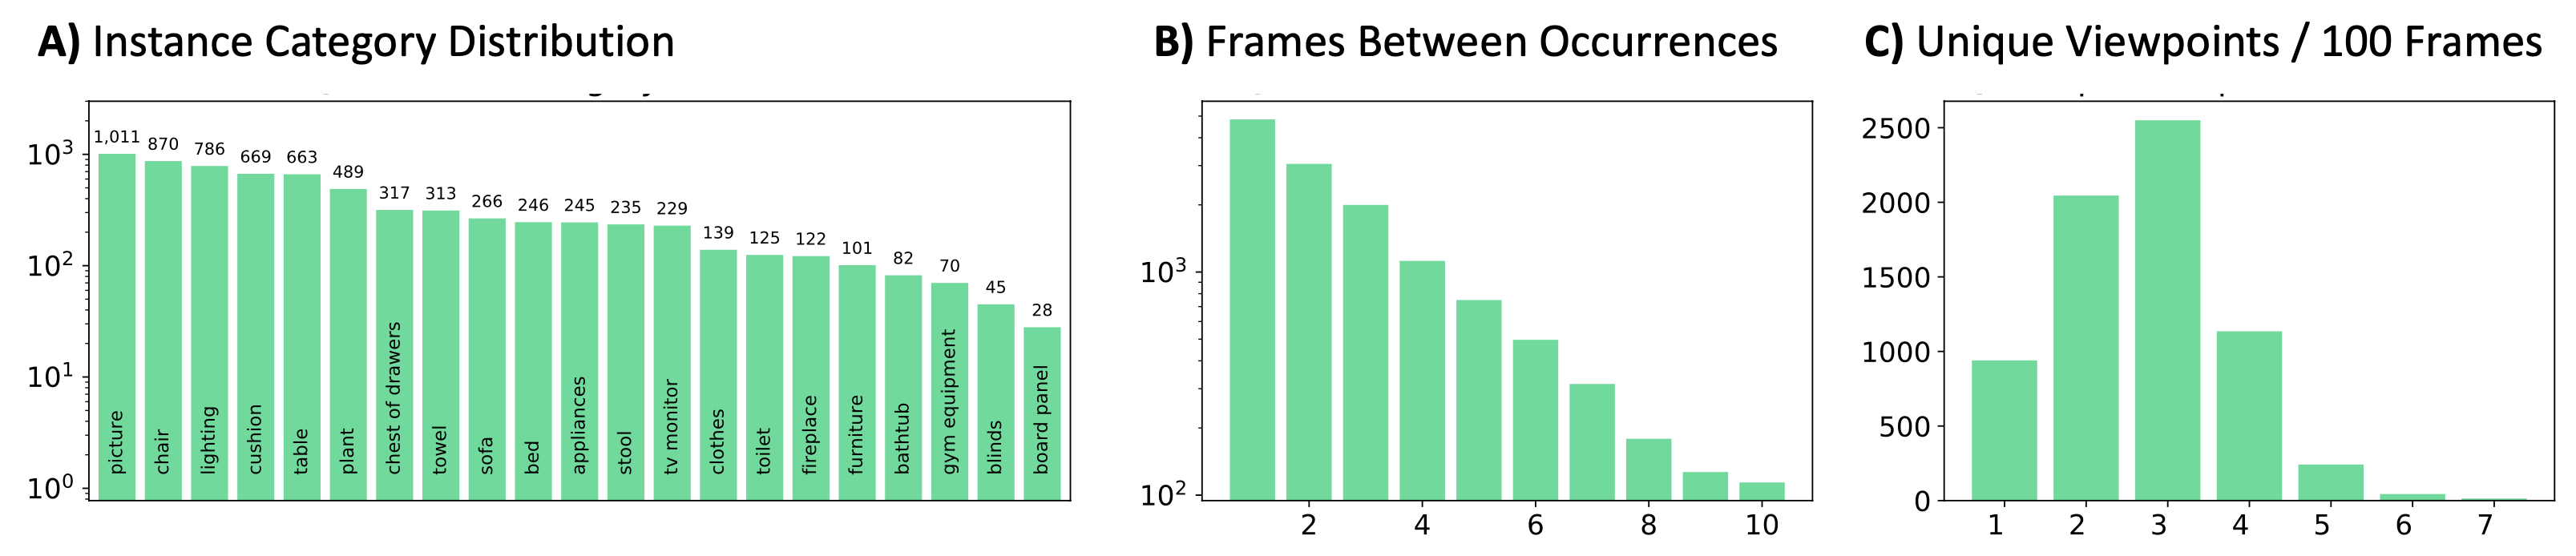
\includegraphics[width=6\textwidth]{figures/condensedv2.png}
\else
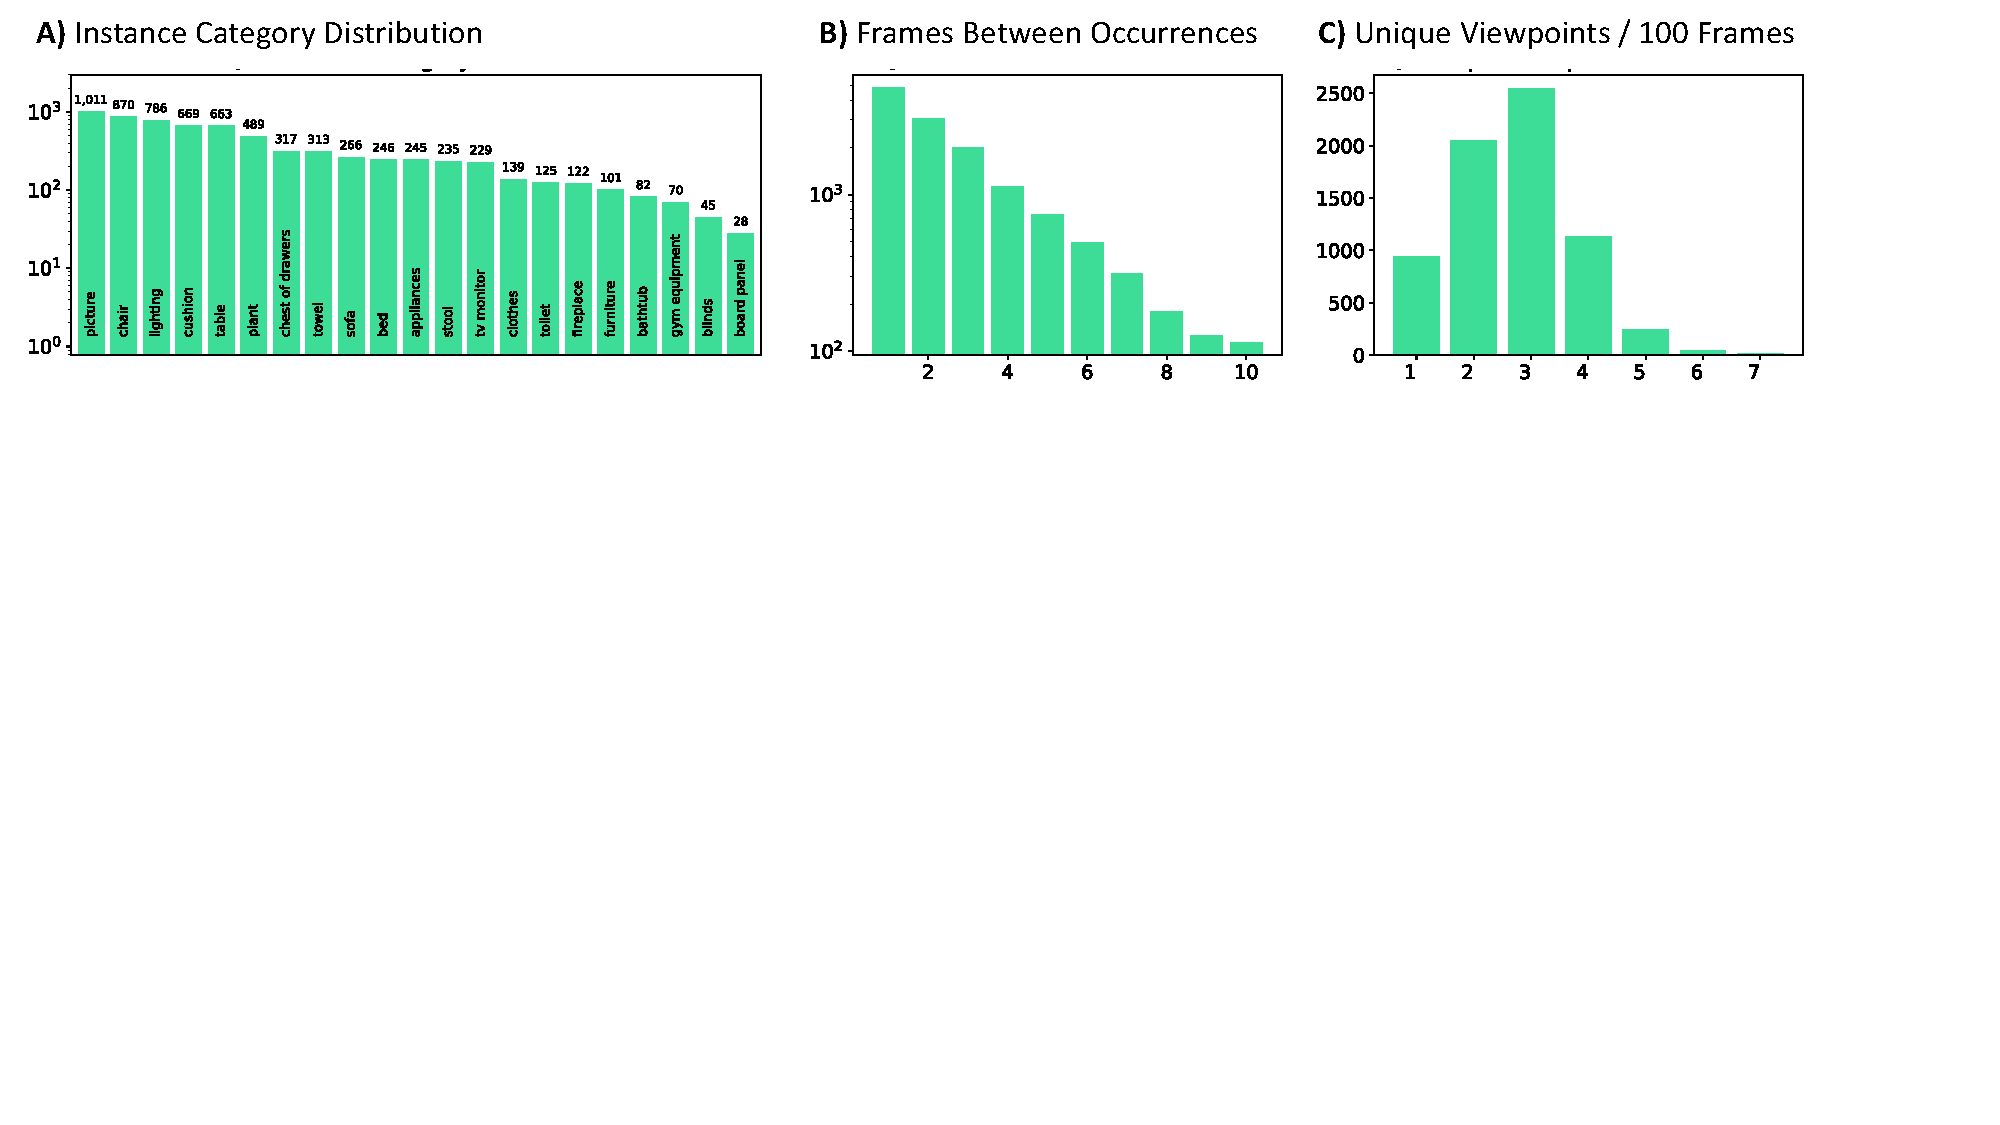
\includegraphics[width=\textwidth,trim={0cm 12.5cm 2.5cm 0cm},clip]{figures/condensedv2.pdf}
\fi
\vspace{-.25in}
\caption{\textbf{Statistics for our \ourroom{} dataset.}
Plots show a natural long tail distribution of instances grouped into categories. An
average sequence has 3 different view points. Sequences are highly correlated in time but revisits
are not uncommon. }
\label{fig:dataset_distribution}
\vspace{-0.15in}
\end{figure}

\vspace{-0.1in}
\paragraph{\ourchar{}:}
The Omniglot dataset~\citep{omniglot} contains 1623 handwritten characters from 50 different
alphabets. We split the alphabets into 31 for training, 5 for validation, and 13 for testing. We
augment classes by 90 degree rotations to create 6492 classes in total. Each contextualized few-shot
learning image sequence contains 150 images, drawn from a random sample of 5-10 alphabets, for a
total of 50 classes per sequence. These classes are randomly assigned to 5 different environments;
within an environment, the characters are distributed according to a Chinese restaurant
process~\citep{crp} to mimic the imbalanced long-tail distribution of naturally occurring objects. We
switch between environments using a Markov switching process; i.e., at each step there is a constant
probability of switching to another environment. An example sequence is shown in
Figure~\ref{fig:dataset}-A.

\vspace{-0.1in}
\paragraph{\ourroom{}:}
As none of the current few-shot learning datasets provides the natural online learning experience
that we would like to study, we created our own dataset using simulated indoor environments. We
formulate this as a few-shot instance learning problem, which could be a use case for a home robot:
it needs to quickly recognize and differentiate novel object instances, and large viewpoint
variations can make this task challenging (see examples in Figure~\ref{fig:dataset}-B). There are
over 7,000 unique instance classes in the dataset, making it suitable to meta-learning approaches.

Our dataset is derived from the Matterport3D dataset~\citep{matterport} with 90 indoor worlds
captured using panoramic depth cameras. We split these into 60 worlds for training, 10 for
validation and 20 for testing. MatterSim~\citep{mattersim} is used to load the simulated world and
collect camera images and HabitatSim~\citep{habitat} is used to project instance
segmentation labels onto 2D image space. We created a random walking agent to collect the virtual
visual experience. For each viewpoint in the random walk, we randomly sample one object from
the image sensor and highlight it with the available instance segmentation, forming an input {\it
frame}. Each viewpoint provides environmental context---the other objects present in the
room with the highlighted object.

Figure~\ref{fig:dataset_distribution}-A shows the object instance distribution. We see strong
temporal correlation, as 30\% of the time the same instance appears in the next frame
(Figure~\ref{fig:dataset_distribution}-B), but there is also a significant proportion of revisits.
On average, there are three different viewpoints per 100-image sequence
(Figure~\ref{fig:dataset_distribution}-C). Details and other statistics of our proposed datasets are
included in the Appendix.

\vspace{-0.1in}
\paragraph{\ourimg{}:} To make the classification problem more challenging, we also report results 
on \ourimg, which uses the same online sequence sampler as \ourchar{} but applied on the \textit{tiered}-ImageNet 
dataset~\citep{fewshotssl}, a subset of the original ImageNet dataset~\citep{imagenet}.
It contains 608 classes with a total of 779K images of size 84$\times$84.
We use the same split of classes as \citet{fewshotssl}. The high-level categories are used for
sampling different ``environments'' just like the notion of alphabets in \ourchar{}.
